
% !TEX program = xelatex
% !TEX encoding = UTF-8
% ctexart + fontspec 需 XeLaTeX：加此行后 VSCode/TeXstudio/latexmk 会自动选对引擎
% 命令行编译：cd 到本目录后 xelatex 数学建模论文.tex（跑两遍以解析交叉引用）
\documentclass[12pt,a4paper]{ctexart}

% ---------------------------------------------------------------------
% 一、页面与版式
% ---------------------------------------------------------------------
\usepackage[paper=a4paper,margin=3cm]{geometry}   % A4 纸，3cm 边距
\usepackage{indentfirst}                          % 段首缩进两格
\usepackage{float}                                 % [H] 精确浮动控制
\usepackage{fancyhdr}                              % 页眉页脚

% 页眉页脚设置（页码居中底部，去掉页眉横线）
\pagestyle{fancy}
\fancyhf{}
\cfoot{\thepage}
\renewcommand{\headrulewidth}{0pt}

% ---------------------------------------------------------------------
% 二、数学与公式
% ---------------------------------------------------------------------
\usepackage{amsmath,amssymb}   % 数学环境、符号

% ---------------------------------------------------------------------
% 三、图表
% ---------------------------------------------------------------------
\usepackage{graphicx}          % 插入图片
\usepackage{booktabs}          % 三线表（\toprule/\midrule/\bottomrule）
\usepackage{caption}           % 图表标题
\usepackage{subcaption}        % 子图（并排图片）
\usepackage{multirow}          % 表格跨行
\usepackage{tikz}              % 流程图、示意图
\usetikzlibrary{arrows.meta,shapes.geometric,positioning}

% ---------------------------------------------------------------------
% 四、算法与代码
% ---------------------------------------------------------------------
\usepackage{algorithm}         % 算法浮动体
\usepackage{algpseudocode}     % 算法伪代码
\usepackage{xcolor}            % 颜色（代码高亮用）
\usepackage{listings}          % 代码列表
\usepackage{listingsutf8}      % 代码 UTF-8 支持

% Python 代码样式（可按需修改颜色/字号）
\lstdefinestyle{pycode}{
    language=Python,
    inputencoding=utf8,
    extendedchars=true,
    basicstyle=\ttfamily\small,
    numbers=left,
    numberstyle=\scriptsize\color{gray},
    numbersep=6pt,
    keywordstyle=\color{blue}\bfseries,
    keywordstyle={[2]\color{purple}\bfseries},
    commentstyle=\color{teal!60!black}\itshape,
    stringstyle=\color{orange!70!black},
    emph={np,pd,plt,torch,tf},
    emphstyle=\color{violet}\bfseries,
    showstringspaces=false,
    tabsize=4,
    frame=single,
    rulecolor=\color{black!40},
    breaklines=true,
    breakatwhitespace=true,
    keepspaces=true,
    captionpos=t
}
\lstset{style=pycode}

% ---------------------------------------------------------------------
% 五、超链接（务必最后加载）
% ---------------------------------------------------------------------
\usepackage{hyperref}
\hypersetup{colorlinks=true,linkcolor=black,urlcolor=blue,citecolor=black}

% ---------------------------------------------------------------------
% 六、论文引用格式
% ---------------------------------------------------------------------
\usepackage{url}

% =====================================================================
% 正文开始
% =====================================================================
\begin{document}

% 从摘要页开始编号为 1
\pagenumbering{arabic}
\setcounter{page}{1}
\thispagestyle{fancy}

% =====================================================================
% 摘 要 页（占满第一页）
% =====================================================================
\begin{center}
{\LARGE\bfseries 论文标题：在此填写你的论文题目}\\[1.5em]
{\large\bfseries 摘~~要}\\[0.8em]
\end{center}

% 在这里填写你的摘要正文。
% 建议直接粘贴真实摘要文字：
%   - 摘要不足一页时，下面的 \vfill 会把内容推到顶部、底部留白；
%   - 摘要超过一页时，会自然分页。
% 摘要写作要点（供参考，非固定格式）：
%   1. 问题背景与总目标（一两句）；
%   2. 针对问题一/二/三……分别写：用了什么模型、什么算法、得到什么关键结果；
%   3. 关键词。

（摘要正文占位……）

\textbf{针对问题一}，……（模型名）……得到……（关键结论）。

\textbf{针对问题二}，……（模型名）……得到……（关键结论）。

\textbf{针对问题三}，……（模型名）……得到……（关键结论）。

\textbf{针对问题四}，……（模型名）……得到……（关键结论）。

\medskip
关键词:\textbf{关键词1~关键词2~关键词3~关键词4~关键词5}

\vfill
\clearpage
% ---------------- 摘要页结束 ----------------

% =====================================================================
% 章节编号：一级标题用中文数字（一、二、三），二级用阿拉伯数字（1.1）
% =====================================================================
\renewcommand{\thesection}{\chinese{section}}
\renewcommand{\thesubsection}{\arabic{section}.\arabic{subsection}}

% =====================================================================
% 一、问题重述
% =====================================================================
\section{问题重述}
\subsection{问题背景}

中药材干燥是决定成品品质的关键工序之一，热风烘干因其设备简单、操作方便而被广泛采用。
热风烘干过程一般包含\textbf{预热平衡}与\textbf{恒温干燥}两个阶段，通过调控烘房内的温度与
水分浓度（含湿量）环境完成药材的脱水。若工艺参数选取不当，容易出现干燥效率低、能耗高、
成品品质不稳定等问题；而传统的试验优化方法成本高、周期长。因此，需要借助数理分析与数值
仿真手段，建立药材烘干过程中温度场与水分浓度场的变化规律模型，为工艺优化提供依据。本文
以圆柱形中药材为研究对象，在已知烘房温湿度时变环境与药材物性参数的条件下，求解药材内部
温度与水分浓度的时空分布，并进一步确定满足干燥指标所需的烘干时间。

\subsection{问题提出}

在不改变原题意的前提下，将赛题重述为如下四个子问题：

\begin{enumerate}
    \item \textbf{问题一（预热平衡阶段建模与求解）}：对于长 $25\ \mathrm{cm}$、半径
    $2\ \mathrm{cm}$ 的圆柱形药材，烘干开始时温度为 $28\ ^\circ\mathrm{C}$、水分浓度
    （干基含水率）为 $2.55\ \mathrm{kg/kg}$。在附件1给出的烘房温度与水分浓度时变环境下，
    建立预热平衡阶段药材温度与水分浓度变化规律的数学模型（物性参数见附录2），并按表1、表2
    格式给出 $100\sim1800\ \mathrm{s}$ 内若干指定时刻、距药材中心 $0\sim2\ \mathrm{cm}$
    处的温度与水分浓度，完整结果按要求保存至 result1.xlsx，所有结果保留四位小数。
    \item \textbf{问题二（整个烘干过程建模与求解）}：烘干过程通常持续 $2\sim3$ 天，
    预热平衡与恒温干燥两阶段的工艺参数有所不同。建立整个烘干过程中药材温度与水分浓度变化
    规律的数学模型（经验公式统一采用附录3），并按表3、表4格式给出前 $3\ \mathrm{h}$ 内
    每隔 $0.5\ \mathrm{h}$、距药材中心 $0\sim2\ \mathrm{cm}$ 处的温度与水分浓度，完整结果
    保存至 result2.xlsx。
    \item \textbf{问题三（满足含水率指标的烘干时间）}：以药材各处水分浓度均不高于
    $0.15\ \mathrm{kg/kg}$ 作为干燥达标的判据，确定药材烘干所需的总时间（单位：$\mathrm{h}$），
    并按表5格式给出每隔 $6\ \mathrm{h}$、距药材中心每隔 $0.5\ \mathrm{cm}$ 处的水分浓度，
    完整结果保存至 result3.xlsx。
    \item \textbf{问题四（考虑尺寸收缩的烘干时长）}：实际烘干过程中，药材会因水分流失
    而发生尺寸变化。在考虑该尺寸变化（附件2）的前提下，采用附录4的经验公式重新确定药材的
    烘干时长，并按表6格式给出每隔 $6\ \mathrm{h}$、距药材中心每隔 $0.5\ \mathrm{cm}$ 处的
    水分浓度，完整结果保存至 result4.xlsx。
\end{enumerate}

% =====================================================================
% 二、问题分析
% =====================================================================
\section{问题分析}
本文研究圆柱形中药材在热风烘干过程中温度场与水分浓度场的时空演化规律。四个子问题由浅入深、
层层递进：问题一建立预热平衡阶段的基础传热--传质模型；问题二将其推广至持续 $2\sim3$ 天的
完整烘干过程，并引入随温湿度变化的物性参数；问题三在问题二模型的基础上确定满足含水率指标的
烘干时间；问题四进一步考虑水分流失引起的尺寸收缩，将固定域问题推广为移动边界问题。下面逐一分析。

\subsection{问题一的分析}
问题一属于典型的\textbf{非稳态传热--传质}问题，在数学上归结为圆柱域上一组抛物型偏微分方程的
初边值问题。其难点主要有二：其一，药材长径比很大（$L/R=12.5$），直接进行三维瞬态求解代价
过高，需要作几何降维；其二，烘房温度与空气含湿量是时变边界条件，且实测数据存在测量噪声，
需先平滑处理。

\textbf{建模思路}：由于 $L\gg R$，忽略轴向端部效应与周向不均匀性，将圆柱药材退化为
\textbf{无限长圆柱}，问题降维为一维径向问题，仅研究 $r\in[0,R]$。温度场由 Fourier 热传导
定律描述，水分场由 Fick 第二定律描述；中心轴处由轴对称性给出诺伊曼零通量条件，表面处由
对流换热与对流传质给出 Robin 型边界条件，环境时变量 $T_a(t)$、$C_a(t)$ 取自附件1并经
Savitzky--Golay 平滑。

\textbf{求解思路}：附录2 中 $\rho,c_p,k,h,h_m$ 均为常数，扩散系数 $D$ 仅依赖水分浓度 $C$
而与温度 $T$ 无关，故传热方程与传质方程相互\textbf{解耦}，可分别独立求解。空间方向采用
\textbf{有限体积法}（守恒形式）离散，时间方向采用 \textbf{Crank--Nicolson} 格式（二阶精度、
无条件稳定）；传质方程因 $D(C)$ 非线性，每步采用 \textbf{Picard 迭代}（滞后系数）线性化。
最终按表1、表2给出指定时刻、指定径向位置的结果，并将完整结果保存至 result1.xlsx。

\subsection{问题二的分析}
问题二将研究范围由 $30$ 分钟的预热阶段扩展到持续 $2\sim3$ 天的\textbf{完整烘干过程}，
涵盖预热平衡与恒温干燥两个阶段。相较问题一，其本质区别体现在四点：

其一，\textbf{物性参数随状态变化}。附录3给出密度 $\rho=650+128C$、比热容
$c_p=1450+2736\,C/(C+1)$、热传导系数 $k=0.21+0.38\,C/(C+1)$ 均随水分浓度 $C$ 变化，
扩散系数 $D=2.4\times10^{-3}e^{-0.45/C}e^{-3850/T}$ 同时依赖 $C$ 与温度 $T$（含 Arrhenius 型
温度项）。这使得 $\rho,c_p$ 不再能提到时间导数外，传热方程与传质方程\textbf{双向耦合}，
需联立求解，不能再如问题一那样解耦。

其二，\textbf{几何不能再降维}。问题一将药材退化为无限长圆柱，依据是 $30\ \mathrm{min}$ 的
预热时间尺度远小于轴向扩散的特征时间；而恒温干燥阶段持续数天，轴向端面的对流交换会经轴向
扩散逐步向内部渗透，端部效应不再可以忽略。同时物性随 $C,T$ 变化，方程也不再具有严格的轴对称
简化依据。因此问题二需在柱坐标下建立\textbf{完整三维模型}，径向、周向、轴向的控制体与通量
均实际保留，以严格反映各控制体真实的通量与边界面积。

其三，\textbf{两阶段的衔接时刻需识别}。预热平衡与恒温干燥的物性公式并不相同，但两者的分界
时刻 $t_c$ 题目中并未直接给出，需依据附件1的实测温度数据判定。若采用单一温度阈值，容易被
测温噪声提前触发，也无法保证此后烘房确实保持恒温，故需构造同时考察“接近平台”与“升温速率
足够小”、并附加持续性要求的判据。

其四，\textbf{环境条件需外推，时间尺度跨度大}。附件1仅覆盖前 $4\ \mathrm{h}$
（$14400\ \mathrm{s}$），其平台均值 $\overline{T}_a\approx50\ ^\circ\mathrm{C}$、
$\overline{C}_a\approx0.05\ \mathrm{kg/kg}$ 可作为此后恒温干燥阶段的稳态环境输入。预热阶段
约 $1.9\ \mathrm{h}$（$6780\ \mathrm{s}$），而整个干燥过程长达 $2\sim3$ 天，物性参数通过
$C$、$T$ 缓慢演化，需兼顾数值稳定性与长期仿真的计算效率。

\textbf{求解思路}：由于不能降维且两方程双向耦合，问题二在\textbf{三维柱坐标有限体积框架}下
求解——每个控制体按 $r\Delta r\Delta\varphi\Delta z$ 精确计算体积，面通量用\textbf{调和平均}
折算导率，边界控制体保留半网格内部阻力与外部对流阻力的串联。两阶段物性按识别出的 $t_c$
分段取用，$t_c$ 处只切换物性、状态量继承前一步的结果以保证连续；时间方向采用\textbf{隐式
（后向欧拉）推进}，每步用 \textbf{Picard 迭代}更新温度、含水率及物性直至收敛。按表3、表4
输出前 $3\ \mathrm{h}$ 内每隔 $0.5\ \mathrm{h}$、距中心 $0,0.5,1,1.5,2\ \mathrm{cm}$ 处的结果，
完整结果保存至 result2.xlsx。

\subsection{问题三的分析}
问题三在问题二完整模型的基础上引入\textbf{干燥达标判据}：药材各处水分浓度均不高于
$C_{\mathrm{crit}}=0.15\ \mathrm{kg/kg}$。由于圆柱药材的水分浓度沿径向由外向内递增，
中心 $r=0$ 处水分浓度最高、下降最慢，故“各处均 $\le0.15$”等价于“中心含水率
$C(0,t)\le0.15$”。由此，多维达标判断归结为对中心点时间序列的监控，问题转化为一个
\textbf{临界时间的确定}问题。

\textbf{求解思路}：在问题二模型上作长时间推进，定时检测 $\max C$；当首次满足达标条件时
终止，该时刻即为烘干总时长。为精确定位达标时刻，可先以较粗步长推进至接近达标，再通过
\textbf{二分或插值}细化。按表5格式每隔 $6\ \mathrm{h}$、径向每隔 $0.5\ \mathrm{cm}$ 输出
水分浓度，完整结果每隔 $60\ \mathrm{s}$ 保存至 result3.xlsx。

\subsection{问题四的分析}
问题四考虑实际烘干中因水分流失导致的\textbf{尺寸收缩}，是前三个问题的进一步扩展。附件2
给出药材半径随时间的变化数据（$0\sim72\ \mathrm{h}$ 内 $R$ 由 $2.0\ \mathrm{cm}$ 收缩至约
$1.2\ \mathrm{cm}$），即求解域外边界 $R(t)$ 随时刻\textbf{移动}，构成移动边界（动边界）
问题；同时物性参数改用附录4的经验公式（其系数与附录3不同）。

难点在于：半径收缩使空间离散域逐时刻变化，固定网格难以直接套用；移动边界上水分通量的处理
需与收缩速率协调；表6要求输出到“药材表面”的水分浓度，而该位置本身随时刻移动。

\textbf{求解思路}：采用\textbf{坐标变换（Landau 变换 $\xi=r/R(t)$）}将移动区间 $[0,R(t)]$
映射到固定区间 $[0,1]$，把动边界问题转化为含由 $R'(t)$ 引起的对流项的固定域方程，再沿用
问题三的数值框架求解；由附件2数据插值或拟合得到 $R(t)$。据此重新确定烘干时长，并按表6
输出水分浓度，完整结果保存至 result4.xlsx。

% =====================================================================
% 三、模型假设
% =====================================================================
\section{模型假设}
% 列出建模所需的合理假设，用编号列表。
\begin{enumerate}
    \item 假设一……
    \item 假设二……
    \item 假设三……
\end{enumerate}

% =====================================================================
% 四、符号说明
% =====================================================================
\section{符号说明}
本文用到的主要符号及其含义、单位见表~\ref{tab:symbols}。除特别说明外，各符号在四个问题中
含义一致。

\begin{table}[H]
\centering
\small
\begin{tabular}{lll}
\toprule
符号 & 含义 & 单位 \\
\midrule
$t$ & 时间 & $\mathrm{s}$（部分结果用 $\mathrm{h}$） \\
$r$ & 径向坐标，到药材中心的距离 & $\mathrm{m}$（结果表用 $\mathrm{cm}$） \\
$\xi$ & 归一化径向坐标 $\xi=r/R(t)$（问题四） & — \\
$R$ & 药材半径 & $\mathrm{m}$ \\
$R(t)$ & 收缩后的药材半径（问题四） & $\mathrm{m}$ \\
$L$ & 药材长度 & $\mathrm{m}$ \\
$T(r,t)$ & 药材内部温度 & $^\circ\mathrm{C}$（附录公式用 $\mathrm{K}$） \\
$C(r,t)$ & 药材水分浓度（干基含水率） & $\mathrm{kg/kg}$ \\
$T_a(t)$ & 烘房环境温度 & $^\circ\mathrm{C}$ \\
$C_a(t)$ & 烘房空气含湿量 & $\mathrm{kg/kg}$ \\
$T_0$ & 药材初始温度 & $^\circ\mathrm{C}$ \\
$C_0$ & 药材初始水分浓度 & $\mathrm{kg/kg}$ \\
$C_{\mathrm{crit}}$ & 干燥达标含水率 & $\mathrm{kg/kg}$ \\
$\rho$ & 药材密度 & $\mathrm{kg/m^3}$ \\
$c_p$ & 药材比热容 & $\mathrm{J/(kg\cdot K)}$ \\
$k$ & 热传导系数 & $\mathrm{W/(m\cdot K)}$ \\
$h$ & 对流换热系数 & $\mathrm{W/(m^2\cdot K)}$ \\
$h_m$ & 对流传质系数 & $\mathrm{m/s}$ \\
$D$ & 水分扩散系数 & $\mathrm{m^2/s}$ \\
$\alpha$ & 热扩散系数 $\alpha=k/(\rho c_p)$ & $\mathrm{m^2/s}$ \\
$Bi_m$ & 传质毕渥数 $Bi_m=h_mR/D$ & — \\
$N$ & 径向网格节点数 & — \\
$\Delta r$ & 径向空间步长 & $\mathrm{m}$ \\
$\Delta t$ & 时间步长 & $\mathrm{s}$ \\
$t_{\mathrm{dry}}$ & 烘干总时长（问题三、四） & $\mathrm{h}$ \\
\bottomrule
\end{tabular}
\caption{符号说明}
\label{tab:symbols}
\end{table}

% =====================================================================
% 五、模型的建立与求解（每个问题一节，按需增减）
% =====================================================================
\section{问题一模型的建立与求解}
\subsection{问题一模型的建立}

\textbf{1. 数据预处理与边界条件}

模型求解所需的烘房环境条件由附件1给出：共 $241$ 个采样点，时间范围 $t\in[0,14400]\ \mathrm{s}$、
采样间隔 $60\ \mathrm{s}$，记录了预热平衡阶段烘房温度 $T_a(t)$ 与空气含湿量 $C_a(t)$ 的时变
数据。实测平台段温度存在测量噪声（$t\ge10800\ \mathrm{s}$ 段标准差约 $0.153\ ^\circ\mathrm{C}$），
直接逐点连线会引入锯齿状波动，故采用 Savitzky--Golay 保形滤波（窗宽 $31$ 点即 $31\ \mathrm{min}$、
三阶多项式）对全段数据平滑：平台段温度标准差降至 $0.027\ ^\circ\mathrm{C}$（降幅约 $82\%$），
平台均值偏差 $3.2\times10^{-4}\ ^\circ\mathrm{C}$，可忽略；同时上升段拐点得以保留——前
$30\ \mathrm{min}$ 内平滑前后最大差异 $0.17\ ^\circ\mathrm{C}$，仅为该时段升温幅度
（$13.5\ ^\circ\mathrm{C}$）的 $1.3\%$。平滑后的 $T_a(t)$、$C_a(t)$ 经线性插值后，作为问题一、
问题二对流边界条件中环境温度与空气含湿量的输入。

图~\ref{fig:boundary} 给出问题一计算区间（前 $30\ \mathrm{min}$）内烘房温度与空气含湿量的
逐点变化：圆点为原始采样点，实线为经 Savitzky--Golay 平滑后用于对流边界条件的曲线。
由附件1 的全部 $241$ 个采样点可知：烘房温度由
$28\ ^\circ\mathrm{C}$ 线性升温至恒温段平台（平台均值 $\overline{T}_a\approx 49.9966\ ^\circ\mathrm{C}$），
约在 $t\approx 5160\ \mathrm{s}$（$1.43\ \mathrm{h}$）进入平台；空气含湿量由
$0.01963\ \mathrm{kg/kg}$ 升至恒温段平台（平台均值 $\overline{C}_a\approx 0.04997\ \mathrm{kg/kg}$），
约在 $t\approx 6900\ \mathrm{s}$（$1.92\ \mathrm{h}$）进入平台。上述平台均值可作为问题二、三中
将环境条件外推至 $4\ \mathrm{h}$ 之后恒温干燥阶段的依据；时变段数据经线性插值后，作为问题一对流
边界条件中环境温度 $T_a(t)$ 与空气含湿量 $C_a(t)$ 的输入。

\begin{figure}[H]
\centering
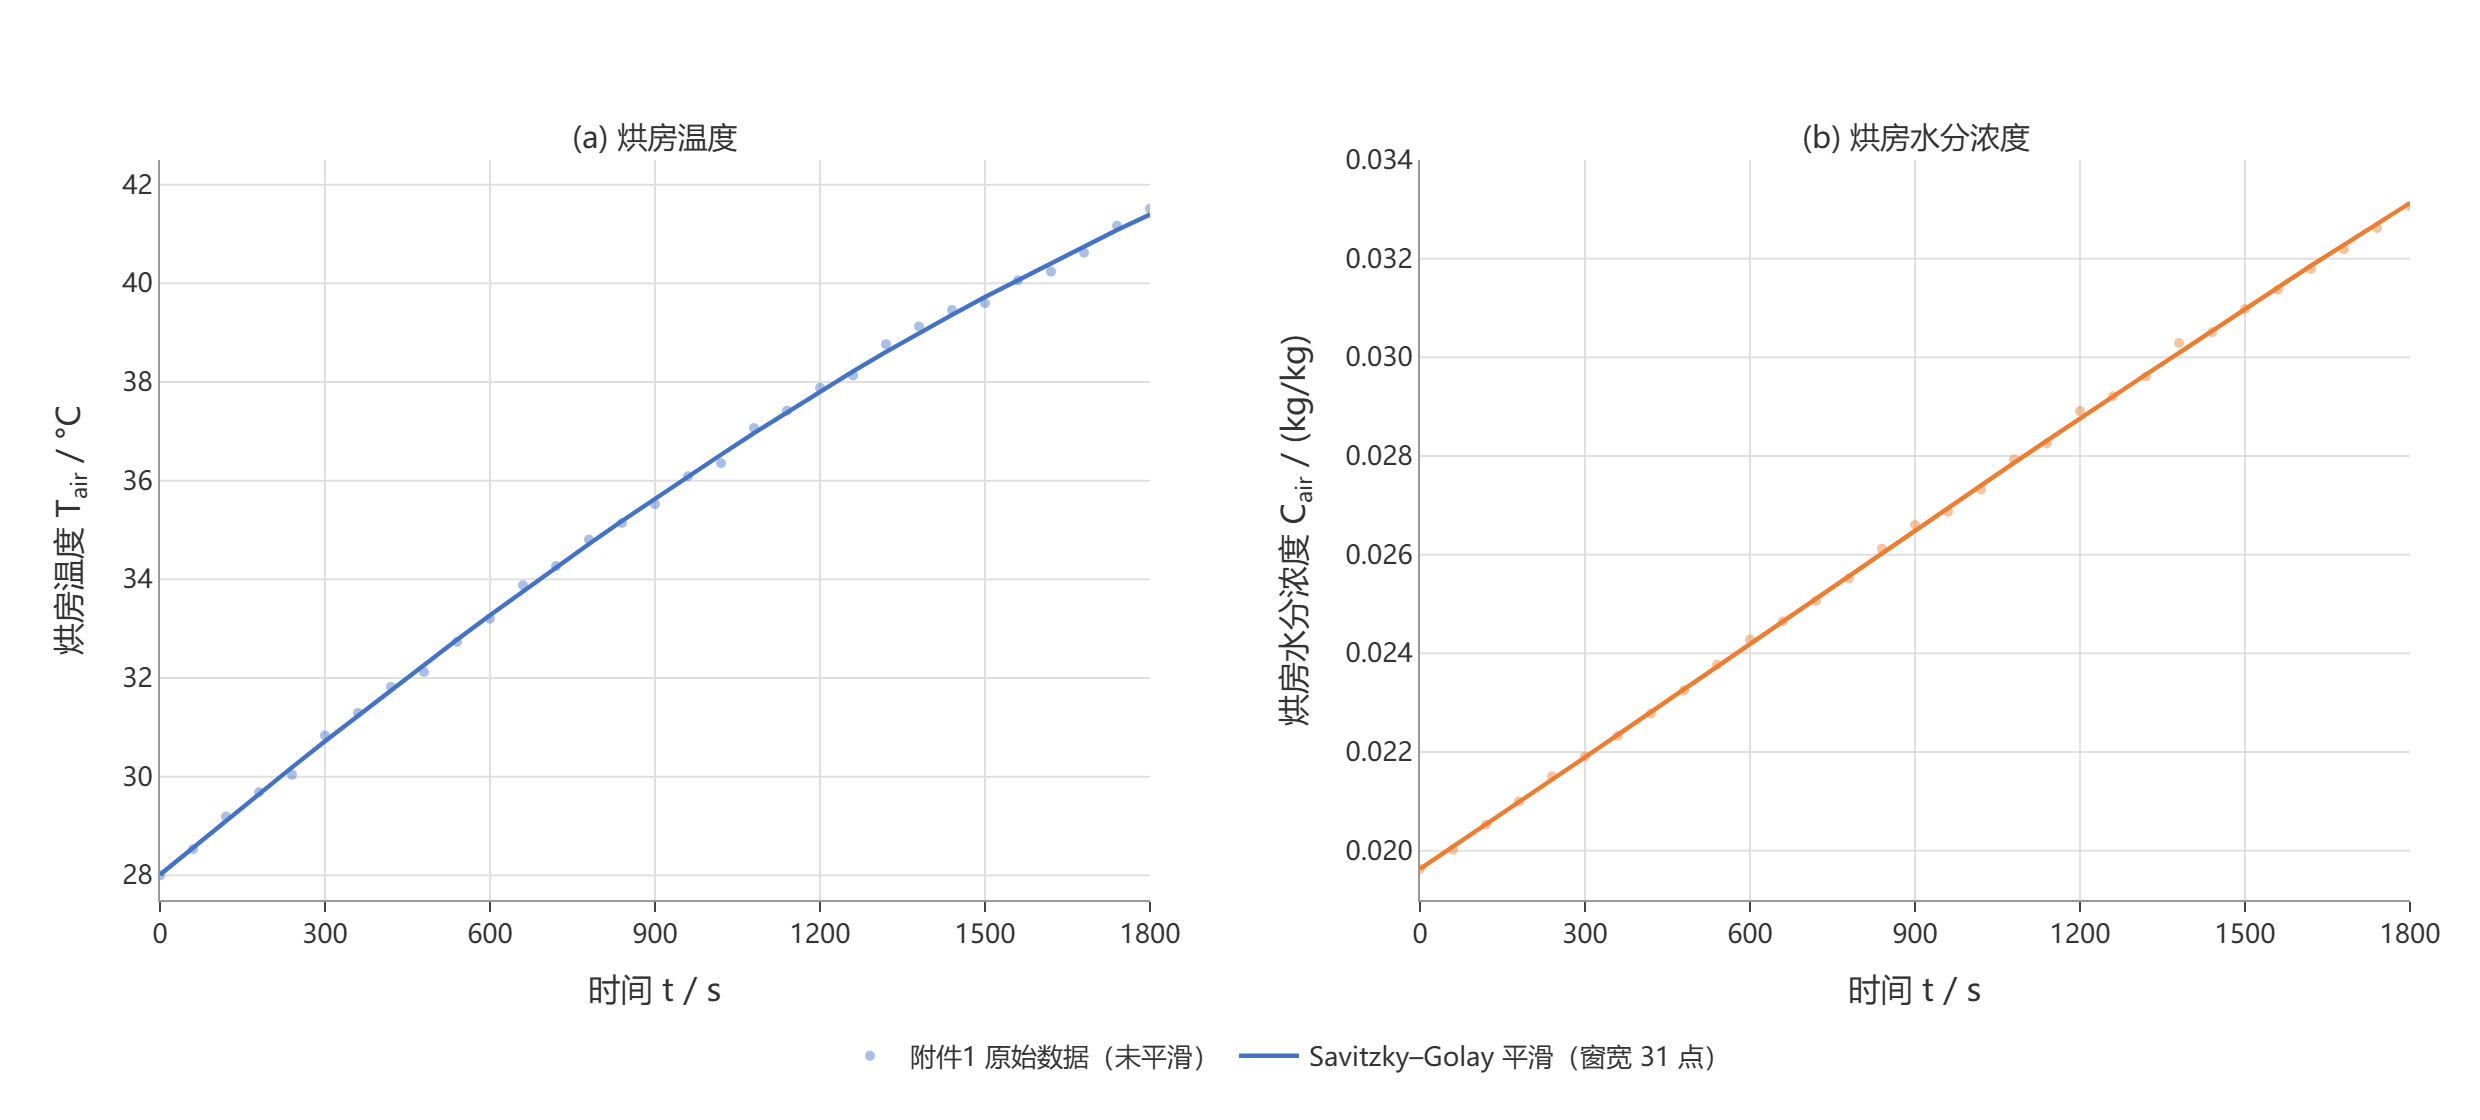
\includegraphics[width=\textwidth]{graphics/fig_q1_boundary_air.png}
\caption{前 $30\ \mathrm{min}$（问题一计算区间）烘房温度与空气含湿量的变化：圆点为附件1 原始采样点
（$60\ \mathrm{s}$ 间隔），实线为 Savitzky--Golay 保形滤波结果（窗宽 $31$ 点）}
\label{fig:boundary}
\end{figure}

\textbf{2. 问题描述与几何简化}

预热平衡阶段，某圆柱形中药材（长 $L=25\ \mathrm{cm}$、半径 $R=2\ \mathrm{cm}$）置于烘房内，
初始温度 $T_0=28\ ^\circ\mathrm{C}$、初始水分浓度（干基含水率）$C_0=2.55\ \mathrm{kg/kg}$。
烘房温度 $T_a(t)$ 与空气含湿量 $C_a(t)$ 随时间的非稳态变化由附件1给出。
由于 $L\gg R$，忽略轴向端部效应，将药材视为\textbf{无限长圆柱}，问题退化为一维径向问题，
仅研究 $r\in[0,R]$ 方向的温度场与水分浓度场。

\textbf{3. 控制方程}

考虑药材内部的传热与传质过程。由于药材可近似视为圆柱体，且其长径比较大，因此忽略轴向温度梯度和水分梯度，并假设温度场与水分迁移过程均具有轴对称性。设 $T(r,t)$ 为时刻 $t$、径向位置 $r$ 处的温度，$C(r,t)$ 为时刻 $t$、径向位置 $r$ 处的水分浓度。

对于药材内部的热传递过程，根据 Fourier 热传导定律，并参考圆柱形物料干燥过程中的热质耦合模型~\cite{ref1}，在上述假设下，可得到圆柱坐标系下的径向一维非稳态热传导方程：

\begin{equation}
\rho c_p\frac{\partial T}{\partial t}
=\frac{k}{r}\frac{\partial}{\partial r}\left(r\frac{\partial T}{\partial r}\right),
\quad 0<r<R,\ t>0
\label{eq:heat}
\end{equation}

其中，$\rho$ 为药材密度，$c_p$ 为比热容，$k$ 为导热系数。
对于药材内部的水分迁移过程，根据 Fick 第二定律及扩散理论~\cite{ref3}，并参考圆柱形物料干燥过程中的传质模型~\cite{ref1}，在考虑有效扩散系数随水分浓度变化的情况下，建立水分传递方程。根据圆柱坐标系下梯度与散度算子的坐标变换关系~\cite{ref2}，并结合轴对称条件，可得到径向一维水分传递方程：
\begin{equation}
\frac{\partial C}{\partial t}
=\frac{1}{r}\frac{\partial}{\partial r}\left(r\,D(C)\frac{\partial C}{\partial r}\right),
\quad 0<r<R,\ t>0
\label{eq:mass}
\end{equation}

\begin{equation}
D(C)=7\times10^{-9}\,e^{-0.89/C}\quad(\mathrm{m^2/s}).
\label{eq:D}
\end{equation}

\textbf{4. 初始条件与边界条件}

初始时刻药材内部温度、水分浓度均匀：
\begin{equation}
T(r,0)=T_0,\qquad C(r,0)=C_0.
\label{eq:ic}
\end{equation}

中心 $r=0$ 处由对称性得：
\begin{equation}
\left.\frac{\partial T}{\partial r}\right|_{r=0}=0,\qquad
\left.\frac{\partial C}{\partial r}\right|_{r=0}=0.
\label{eq:bc_center}
\end{equation}

表面 $r=R$ 处为对流换热与对流传质边界：
\begin{equation}
-k\left.\frac{\partial T}{\partial r}\right|_{r=R}=h\bigl[T(R,t)-T_a(t)\bigr],
\label{eq:bc_heat}
\end{equation}
\begin{equation}
-D\left.\frac{\partial C}{\partial r}\right|_{r=R}=h_m\bigl[C(R,t)-C_a(t)\bigr].
\label{eq:bc_mass}
\end{equation}

\textbf{5. 模型参数}

由附录2，相关物性参数取值见表~\ref{tab:param}。

\begin{table}[H]
\centering
\begin{tabular}{lcl}
\toprule
参数 & 符号 & 数值 \\
\midrule
密度 & $\rho$ & $820\ \mathrm{kg/m^3}$ \\
比热容 & $c_p$ & $2600\ \mathrm{J/(kg\cdot K)}$ \\
热传导系数 & $k$ & $0.36\ \mathrm{W/(m\cdot K)}$ \\
对流换热系数 & $h$ & $25\ \mathrm{W/(m^2\cdot K)}$ \\
对流传质系数 & $h_m$ & $8\times10^{-7}\ \mathrm{m/s}$ \\
初始温度 & $T_0$ & $28\ ^\circ\mathrm{C}$ \\
初始水分浓度 & $C_0$ & $2.55\ \mathrm{kg/kg}$ \\
\bottomrule
\end{tabular}
\caption{问题一相关参数（附录2）}
\label{tab:param}
\end{table}

需要指出，本问中 $\rho,c_p,k,h,h_m$ 均为常数，扩散系数 $D$ 仅依赖 $C$ 而与 $T$ 无关，
故传热方程 \eqref{eq:heat} 与传质方程 \eqref{eq:mass} 相互\textbf{解耦}，可分别独立求解。

\subsection{问题一模型的求解}
\textbf{1. 数值方法}

采用\textbf{有限体积法}（守恒形式）对方程 \eqref{eq:heat}、\eqref{eq:mass} 进行径向空间离散：
将柱坐标散度项写成通量守恒形式，控制体界面取几何坐标 $r_{i\pm1/2}$，得到三对角线性方程组。
时间方向采用 \textbf{Crank--Nicolson} 格式（对线性扩散方程，Crank–Nicolson 格式具有二阶时间精度，并具有良好的稳定性；对于当前含非线性扩散系数的耦合问题，其整体稳定性还需要结合具体离散方程和迭代过程分析~\cite{ref4}。）；由于 $D(C)$ 非线性，
传质方程每步采用 \textbf{Picard 迭代}（滞后系数）求解。环境温湿度 $T_a(t),C_a(t)$ 由附件1数据
经 Savitzky--Golay 平滑后线性插值得到。径向取 $N=1600$ 个节点（$\Delta r=1.25\times10^{-5}\ \mathrm{m}$），
时间步长 $\Delta t=0.25\ \mathrm{s}$。经网格与时间步加密验证，结果变化小于 $10^{-4}$，
满足四位小数精度要求。求解流程见算法~\ref{alg:p1}。

\begin{algorithm}[H]
\caption{问题一瞬态传热--传质数值求解}
\label{alg:p1}
\begin{algorithmic}[1]
\State 初始化：$T\gets T_0$，$C\gets C_0$，径向网格 $r_i=i\Delta r\ (i=0,\dots,N)$
\For{$n=1$ \textbf{to} $M$}
    \State $t_n \gets n\Delta t$；由附件1插值得到环境 $T_a(t_n),\,C_a(t_n)$
    \State 用 Crank--Nicolson 求解温度场 $T^{n}$（解三对角方程）
    \For{$k=1$ \textbf{to} $3$} \Comment{Picard 迭代}
        \State 由 $C^{n,k}$ 计算 $D(C)$，组装并求解水分场 $C^{n,k+1}$
    \EndFor
\EndFor
\State \Return 各时刻、各径向位置的温度 $T$ 与水分浓度 $C$
\end{algorithmic}
\end{algorithm}

\textbf{2. 结果}

按表1、表2格式，给出 $100,300,600,900,1200,1500,1800\ \mathrm{s}$ 时刻、
距中心 $0,0.5,1,1.5,2\ \mathrm{cm}$ 处的温度与水分浓度，见表~\ref{tab:T1}、\ref{tab:C1}。
$1800\ \mathrm{s}$ 内每隔 $1\ \mathrm{s}$、每 $0.1\ \mathrm{cm}$ 的完整结果已保存至 result1.xlsx。
各径向位置的温度与水分浓度随时间的变化曲线见图~\ref{fig:result1}。

\begin{table}[H]
\centering
\begin{tabular}{lccccc}
\toprule
时间/s & 0 & 0.5 & 1.0 & 1.5 & 2.0 \\
\midrule
100 & 28.0001 & 28.0004 & 28.0045 & 28.0347 & 28.1795 \\
300 & 28.0406 & 28.0630 & 28.1511 & 28.3716 & 28.8438 \\
600 & 28.4510 & 28.5338 & 28.8035 & 29.3218 & 30.1837 \\
900 & 29.3243 & 29.4574 & 29.8724 & 30.6132 & 31.7453 \\
1200 & 30.5454 & 30.7133 & 31.2269 & 32.1143 & 33.4157 \\
1500 & 31.9952 & 32.1844 & 32.7574 & 33.7284 & 35.1150 \\
1800 & 33.5711 & 33.7696 & 34.3669 & 35.3667 & 36.7710 \\
\bottomrule
\end{tabular}
\caption{预热平衡阶段药材温度（单位：$^\circ$C；行=时间，列=距中心距离/cm）}
\label{tab:T1}
\end{table}

\begin{table}[H]
\centering
\begin{tabular}{lccccc}
\toprule
时间/s & 0 & 0.5 & 1.0 & 1.5 & 2.0 \\
\midrule
100 & 2.5500 & 2.5500 & 2.5500 & 2.5500 & 2.2471 \\
300 & 2.5500 & 2.5500 & 2.5500 & 2.5492 & 2.0508 \\
600 & 2.5500 & 2.5500 & 2.5500 & 2.5353 & 1.8770 \\
900 & 2.5500 & 2.5500 & 2.5497 & 2.5045 & 1.7547 \\
1200 & 2.5500 & 2.5500 & 2.5482 & 2.4646 & 1.6586 \\
1500 & 2.5500 & 2.5499 & 2.5445 & 2.4206 & 1.5787 \\
1800 & 2.5500 & 2.5497 & 2.5383 & 2.3755 & 1.5102 \\
\bottomrule
\end{tabular}
\caption{预热平衡阶段药材水分浓度（单位：kg/kg；行=时间，列=距中心距离/cm）}
\label{tab:C1}
\end{table}

\begin{figure}[H]
\centering
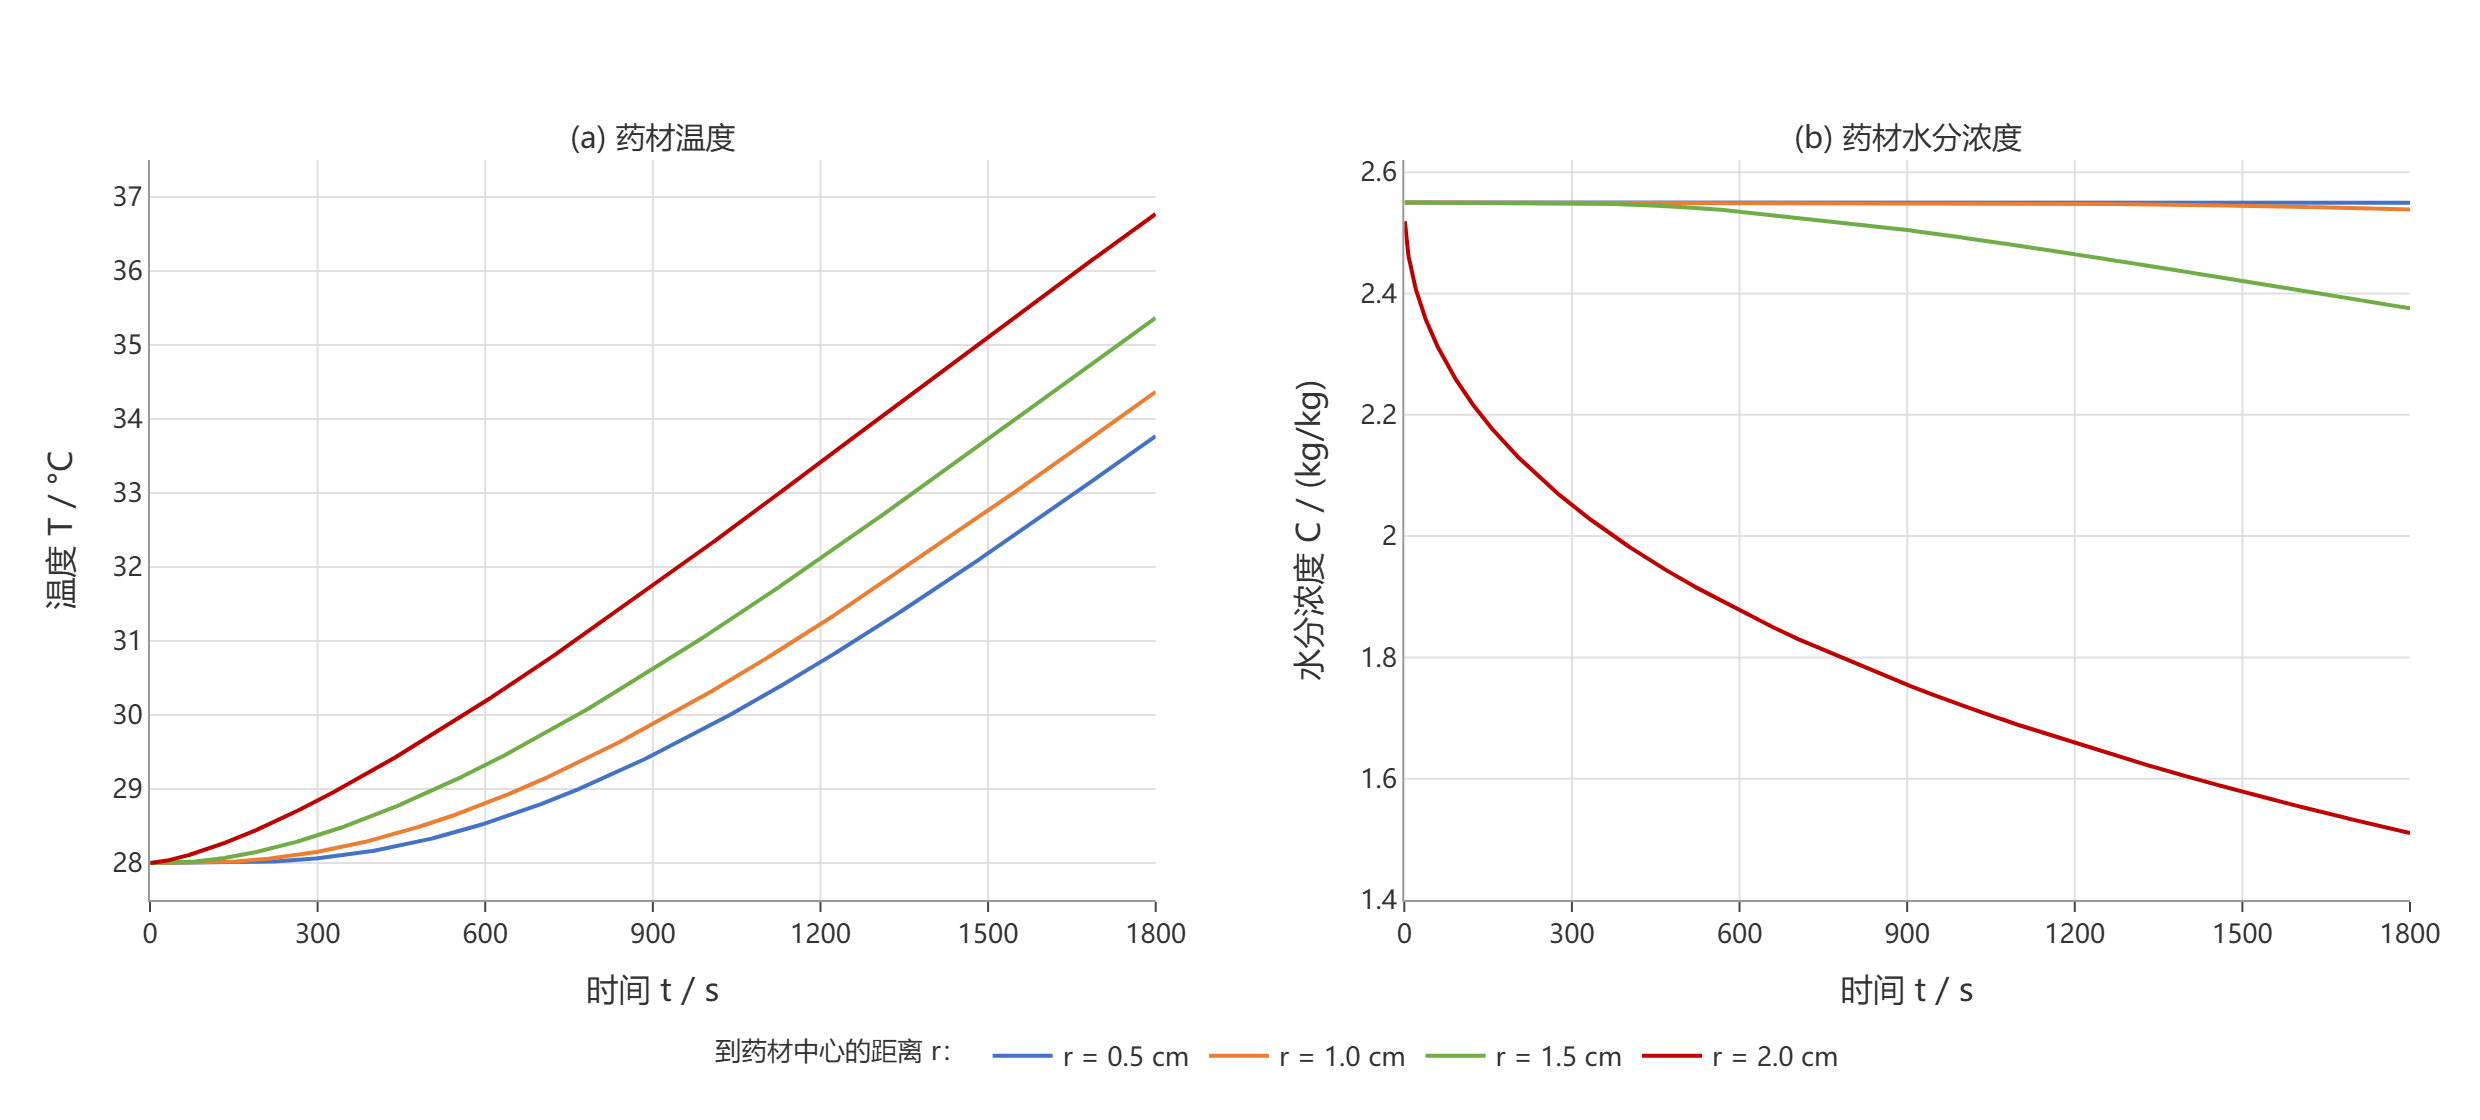
\includegraphics[width=\textwidth]{graphics/fig_q1_curves.png}
\caption{预热平衡阶段药材温度（左）与水分浓度（右）随时间的变化}
\label{fig:result1}
\end{figure}

\textbf{3. 结果分析}

由表~\ref{tab:T1} 可知，药材表面升温较快、中心明显滞后：$1800\ \mathrm{s}$ 时表面已达
$36.77\ ^\circ\mathrm{C}$，而中心仅 $33.57\ ^\circ\mathrm{C}$，径向温差约 $3.2\ ^\circ\mathrm{C}$。
这符合圆柱体热传导的滞后特性——热扩散系数 $\alpha=k/(\rho c_p)\approx1.69\times10^{-7}\ \mathrm{m^2/s}$，
特征时间 $R^2/\alpha\approx2370\ \mathrm{s}$ 大于 $1800\ \mathrm{s}$，故中心尚未充分热透。

由表~\ref{tab:C1} 可知，表面水分浓度由 $2.55\ \mathrm{kg/kg}$ 降至 $1.51\ \mathrm{kg/kg}$，
降幅沿径向由外向内迅速衰减：$r=1.5\ \mathrm{cm}$ 处降至 $2.38\ \mathrm{kg/kg}$，而
$r\le1\ \mathrm{cm}$ 的内部基本保持 $2.55\ \mathrm{kg/kg}$ 不变，呈现明显的“干壳湿芯”特征。
其原因是：传质毕渥数 $Bi_m=h_mR/D(C_0)\approx3.2>1$，外部传质阻力小于内部扩散阻力，故表面
水分浓度能较快跟随环境含湿量下降；而扩散系数
$D(C_0)=7\times10^{-9}e^{-0.89/C_0}\approx4.9\times10^{-9}\ \mathrm{m^2/s}$ 仍然很小，
$30\ \mathrm{min}$ 内水分扩散的特征深度 $\sqrt{Dt}\approx2.9\ \mathrm{mm}$，与表中表面向内约
$1\ \mathrm{cm}$ 的范围内才出现明显失水在量级上一致，更深处的内部尚未受到影响。

% =====================================================================
% 问题二模型的建立与求解
% =====================================================================
\section{问题二模型的建立与求解}

\subsection{问题二模型的建立}

\textbf{1. 分段物性参数与阶段切换}

与问题一仅涉及预热平衡阶段不同，问题二覆盖持续 $2\sim3$ 天的完整烘干过程，预热平衡与恒温
干燥两阶段的物性参数并不相同。按题目要求，经验公式统一采用附录2与附录3，两阶段物性分段
取值见表~\ref{tab:p2param}；扩散系数则分段取为

\begin{equation}
D=\begin{cases}
7\times10^{-9}\,e^{-0.89/C}, & t<t_c,\\[4pt]
2.4\times10^{-3}\,e^{-0.45/C}\,e^{-3850/T}, & t\ge t_c,
\end{cases}
\qquad(\mathrm{m^2/s})
\label{eq:p2D}
\end{equation}

其中 $t_c$ 为两阶段的临界分界时刻，附录3各式中的 $T$ 取热力学温度（单位 K）。

\begin{table}[H]
\centering
\small
\begin{tabular}{lcccc}
\toprule
阶段 & 时间区间 & $\rho\ (\mathrm{kg/m^3})$ & $c_p\ (\mathrm{J/(kg\cdot K)})$ &
$k\ (\mathrm{W/(m\cdot K)})$ \\
\midrule
预热平衡 & $t<t_c$ & $820$ & $2600$ & $0.36$ \\
恒温干燥 & $t\ge t_c$ & $650+128C$ & $1450+2736\dfrac{C}{C+1}$ &
$0.21+0.38\dfrac{C}{C+1}$ \\
\bottomrule
\end{tabular}
\caption{问题二分段物性参数（预热平衡阶段取自附录2，恒温干燥阶段取自附录3）}
\label{tab:p2param}
\end{table}

需要强调的是，恒温干燥阶段的 $\rho,c_p,k$ 均随水分浓度 $C$ 变化，$D$ 同时依赖 $C$ 与温度 $T$
（含 Arrhenius 型温度项）。因此 $\rho,c_p$ 不能再提到时间导数之外，传热方程与传质方程
\textbf{双向耦合}，必须联立求解，这是本问与问题一在模型结构上的本质区别。

\textbf{2. 计算域与三维控制方程}

问题一将药材退化为无限长圆柱，其依据是 $30\ \mathrm{min}$ 的预热时间尺度远小于轴向扩散的
特征时间。但恒温干燥阶段持续数天，轴向端面的对流交换将经轴向扩散逐步向内部渗透，端部效应
不再可以忽略；同时物性随 $C,T$ 变化，方程本身也不再有严格的轴对称简化依据。为严格保留各
控制体的真实通量与边界面积，本问\textbf{不再作降维处理}，直接在柱坐标 $(r,\varphi,z)$ 下
建立完整三维模型~\cite{ref1}。

计算域为整个圆柱体

\begin{equation}
\Omega=\left\{(r,\varphi,z):0\le r\le R,\ 0\le\varphi<2\pi,\
-\tfrac{L}{2}\le z\le\tfrac{L}{2}\right\},
\label{eq:p2domain}
\end{equation}

其中半径 $R=0.02\ \mathrm{m}$、长度 $L=0.25\ \mathrm{m}$，与问题一保持一致。

由能量守恒与质量守恒，控制方程写成守恒（散度）形式

\begin{equation}
\rho c_p\frac{\partial T}{\partial t}=\nabla\cdot(k\nabla T),
\qquad
\frac{\partial C}{\partial t}=\nabla\cdot(D\nabla C).
\label{eq:p2governing}
\end{equation}

利用柱坐标下的梯度与散度算子~\cite{ref2}展开，得径向、周向、轴向三个方向均保留的控制方程

\begin{equation}
\rho c_p\frac{\partial T}{\partial t}
=\frac{1}{r}\frac{\partial}{\partial r}\!\left(rk\frac{\partial T}{\partial r}\right)
+\frac{1}{r^{2}}\frac{\partial}{\partial \varphi}\!\left(k\frac{\partial T}{\partial \varphi}\right)
+\frac{\partial}{\partial z}\!\left(k\frac{\partial T}{\partial z}\right),
\label{eq:p2heat3d}
\end{equation}

\begin{equation}
\frac{\partial C}{\partial t}
=\frac{1}{r}\frac{\partial}{\partial r}\!\left(rD\frac{\partial C}{\partial r}\right)
+\frac{1}{r^{2}}\frac{\partial}{\partial \varphi}\!\left(D\frac{\partial C}{\partial \varphi}\right)
+\frac{\partial}{\partial z}\!\left(D\frac{\partial C}{\partial z}\right).
\label{eq:p2mass3d}
\end{equation}

\textbf{3. 初始条件与边界条件}

初始时刻药材内部温度与水分浓度均匀：

\begin{equation}
T(r,\varphi,z,0)=T_0=28\ ^\circ\mathrm{C},\qquad
C(r,\varphi,z,0)=C_0=2.55\ \mathrm{kg/kg}.
\label{eq:p2ic}
\end{equation}

药材侧面 $r=R$ 与两个端面 $z=\pm L/2$ 均直接暴露于烘房环境，采用对流换热与对流传质条件：

\begin{equation}
-k\left.\frac{\partial T}{\partial n}\right|_{\Gamma}=h\left[T_{\Gamma}-T_a(t)\right],
\qquad
-D\left.\frac{\partial C}{\partial n}\right|_{\Gamma}=h_m\left[C_{\Gamma}-C_a(t)\right],
\label{eq:p2bc}
\end{equation}

其中 $\Gamma$ 表示外边界，$\partial/\partial n$ 为外法向导数，
$h=25\ \mathrm{W/(m^2\cdot K)}$，$h_m=8\times10^{-7}\ \mathrm{m/s}$。周向采用
\textbf{周期性边界}；轴线 $r=0$ 处控制体自然退化，不存在额外的边界面，故无需附加条件。
环境温度与空气含湿量 $T_a(t),C_a(t)$ 由附件1按时间线性插值给出，附件1给定范围之外按
问题一中由附件1确定的恒温段平台值外推。

\textbf{4. 阶段分界时刻 $t_c$ 的稳态统计判定}

分段物性的切换点 $t_c$ 必须依据实测数据客观确定。若采用单一温度阈值（例如烘房温度达到
平台值的 $95\%$ 或 $99.5\%$），容易被测温噪声提前触发，也无法保证此后烘房确实保持恒温。
为此，本文同时检查“接近平台”与“升温速率足够小”两个条件，并附加持续性要求，步骤如下。

\textbf{第 1 步（估计平台）}：用附件1中 $t\ge 10800\ \mathrm{s}$ 的尾段数据估计恒温平台。
需要强调，本步的尾段统计量一律取自\textbf{原始}实测数据——$\sigma$ 应反映真实的测量噪声；
若改用平滑序列的 MAD，量到的只是滤波器自身的平坦度（$\sigma$ 会被压小约 $7$ 倍、稳态带随之
收紧，临界时刻将被人为推迟）。即：\textbf{对流边界条件用平滑序列，阶段判定用原始序列}。
为降低异常波动的影响，平台中心取中位数，噪声尺度取 MAD（中位数绝对偏差）换算的稳健标准差：

\begin{equation}
T^{*}=\operatorname{median}(T_a),\qquad
\sigma=1.4826\cdot\operatorname{median}\left|T_a-T^{*}\right|.
\label{eq:p2mad}
\end{equation}

\textbf{第 2 步（滑动统计量）}：对每个候选时刻 $\tau$，用区间 $[\tau-1200,\ \tau]$（即
$20\ \mathrm{min}$）内的观测值计算滑动均温 $\bar T(\tau)$，并用最小二乘估计升温斜率
$\beta(\tau)$（单位 $^\circ\mathrm{C/min}$）：

\begin{equation}
\bar T(\tau)=\frac{1}{n}\sum_{j=1}^{n}T_a(t_j),\qquad
\beta(\tau)=\frac{\sum_{j}\left(t_j-\bar t\right)\left[T_a(t_j)-\bar T(\tau)\right]}
{\sum_{j}\left(t_j-\bar t\right)^{2}}.
\label{eq:p2slope}
\end{equation}

\textbf{第 3 步（双条件与持续性）}：候选点 $\tau$ 须同时满足

\begin{equation}
\left|\bar T(\tau)-T^{*}\right|\le 2\sigma,
\qquad
\left|\beta(\tau)\right|\le \frac{3\sigma}{20},
\label{eq:p2crit}
\end{equation}

且上述两个条件在 $\tau$ 之后\textbf{连续保持} $1800\ \mathrm{s}$。第一个合格的候选点即定义为
临界时刻 $t_c$。该持续性判断属于离线识别：用后续 $30\ \mathrm{min}$ 的数据确认 $\tau$ 确实
进入稳定段，但将阶段分界\textbf{回标}到 $\tau$；若用于实时控制，则只能在
$\tau+1800\ \mathrm{s}$ 才能确认，不能提前获知未来数据。

由附件1数据计算，各统计量汇总于表~\ref{tab:p2crit}，识别结果为
$t_c=6780\ \mathrm{s}=1.8833\ \mathrm{h}$。

\begin{table}[H]
\centering
\begin{tabular}{lcc}
\toprule
统计量 & 数值 & 含义 \\
\midrule
$T^{*}$ & $50.0030\ ^\circ\mathrm{C}$ & 尾段稳态中位温度 \\
$\sigma$ & $0.2209\ ^\circ\mathrm{C}$ & MAD 换算的稳健波动尺度 \\
$2\sigma$ 温度带 & $\pm0.4418\ ^\circ\mathrm{C}$ & 滑动均温允许偏差 \\
斜率上限 & $0.0331\ ^\circ\mathrm{C/min}$ & 20 分钟窗的趋稳约束 \\
临界窗均温 & $49.5820\ ^\circ\mathrm{C}$ & $\tau=t_c$ 时的 20 分钟均值 \\
临界窗斜率 & $0.0184\ ^\circ\mathrm{C/min}$ & $\tau=t_c$ 时的回归斜率 \\
临界时刻 $t_c$ & $6780\ \mathrm{s}=1.8833\ \mathrm{h}$ & 预热结束、恒温干燥开始 \\
\bottomrule
\end{tabular}
\caption{阶段分界时刻的稳态统计判定结果}
\label{tab:p2crit}
\end{table}

\begin{figure}[H]
\centering
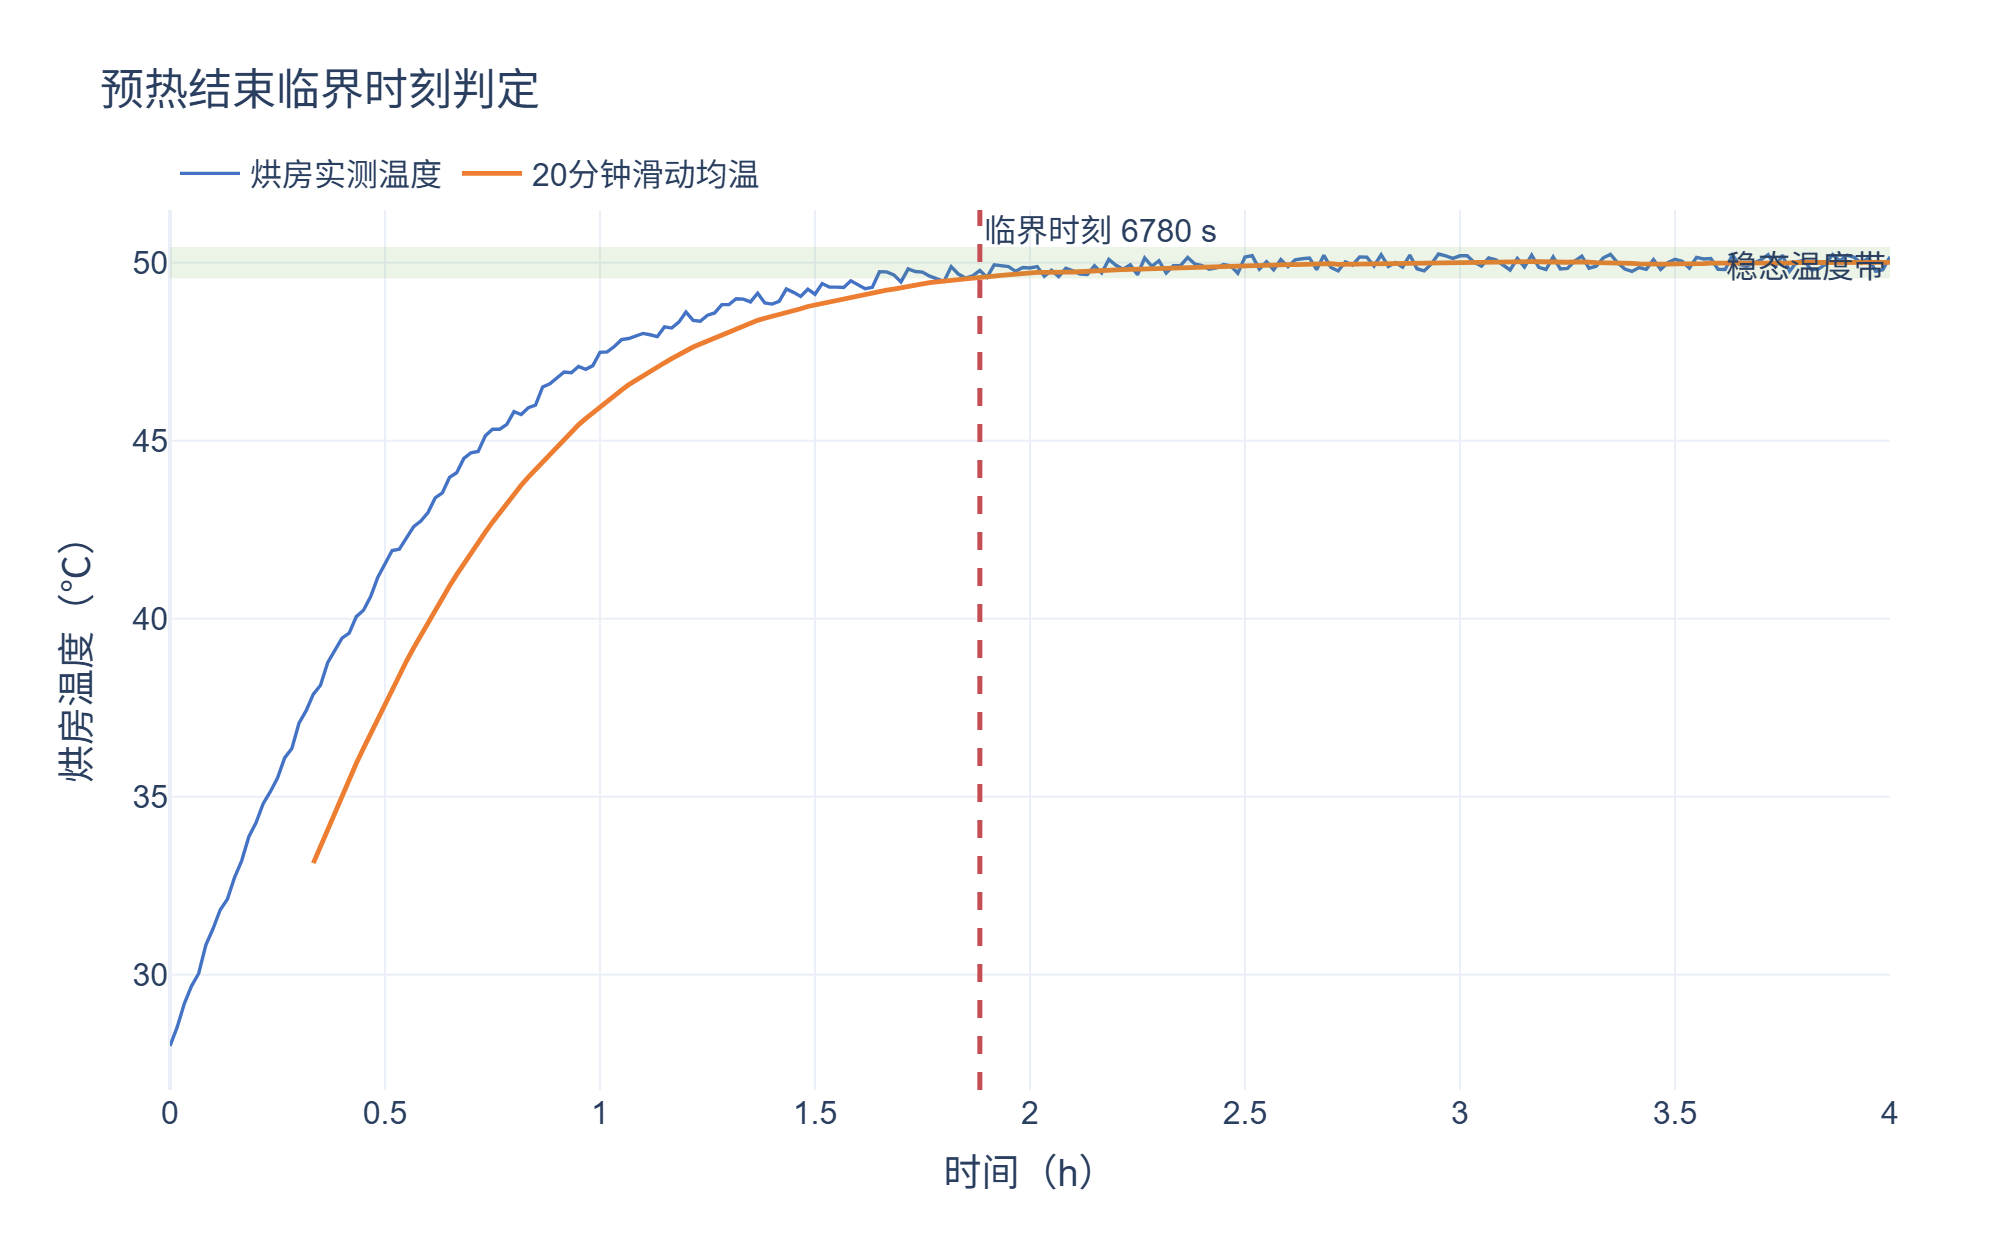
\includegraphics[width=0.92\textwidth]{graphics/fig_q2_critical_time.png}
\caption{预热结束临界时刻判定：绿色带为尾段中位温度与 MAD 给出的稳态温度带，
橙线为 20 分钟滑动均温，红虚线为识别出的临界时刻 $6780\ \mathrm{s}$}
\label{fig:p2crit}
\end{figure}

由图~\ref{fig:p2crit} 可见，滑动均温在 $6780\ \mathrm{s}$ 处进入稳态温度带，升温斜率同时低
于规定上限，并在随后 $30\ \mathrm{min}$ 内持续满足两项条件，故将该点识别为预热结束时刻。该
判据把“是否进入恒温阶段”建立在平台接近程度、升温斜率与持续时间三项证据之上，比单一进度
阈值更能抵抗温度波动。

\textbf{5. 分段物性的连续切换}

临界点处\textbf{只切换物性参数，不重新赋初值}：温度场与水分浓度场在切换处继承前一步的结果，
因而状态连续。数值实现上，若某时间步跨越 $t_c$，程序先把该步\textbf{截断}到 $t_c$，下一步
再启用附录3的物性公式，从而避免把同一个时间步同时解释为两个阶段。这样既保证了物性切换的
物理含义明确，又避免了切换处的数值振荡。

\subsection{问题二模型的求解}

\textbf{1. 数值方法}

采用\textbf{有限体积法}在三维柱坐标控制体上离散方程~\eqref{eq:p2heat3d}、
\eqref{eq:p2mass3d}：径向 $20$、周向 $6$、轴向 $32$，共 $20\times6\times32=3840$ 个控制体，
控制体体积由 $r\Delta r\Delta\varphi\Delta z$ 精确给出，径向、周向、轴向的面通量均按真实
几何面积计算。相邻控制体之间的面通量采用\textbf{调和平均}折算的面导率，以正确反映串联的
导热（扩散）阻力；位于边界的控制体保留半网格内部阻力与外对流阻力串联的等效边界导率，
而非直接以控制体中心值近似表面值。

时间方向采用\textbf{后向欧拉}（隐式）格式，时间步长 $\Delta t=5\ \mathrm{s}$；由于热容
$\rho c_p$ 与扩散系数 $D$ 均随 $C,T$ 变化，每一步内采用 \textbf{Picard 迭代}（滞后系数）
更新温度、水分浓度与物性，收敛判据取

\begin{equation}
\max\left(\frac{\left\|\Delta T\right\|_{\infty}}{50},\
\frac{\left\|\Delta C\right\|_{\infty}}{2.55}\right)<10^{-8},
\label{eq:p2tol}
\end{equation}

即温度与水分浓度的相对变化同时足够小。每一步的线性方程组为对称正定稀疏系统，采用
\textbf{共轭梯度法}配合对角预条件求解。求解流程见算法~\ref{alg:p2}。

\begin{algorithm}[H]
\caption{问题二完整烘干过程三维传热--传质数值求解}
\label{alg:p2}
\begin{algorithmic}[1]
\State 初始化：$T\gets T_0$，$C\gets C_0$，$t\gets 0$，组装三维控制体几何量
\State 由附件1按式~\eqref{eq:p2mad}--\eqref{eq:p2crit} 识别临界时刻 $t_c$
\While{$t<t_{\mathrm{end}}$}
    \State $t_{\mathrm{new}}\gets\min(t+\Delta t,\ t_{\mathrm{end}})$
    \If{$t<t_c<t_{\mathrm{new}}$}
        \State $t_{\mathrm{new}}\gets t_c$ \Comment{时间步截断到阶段分界}
    \EndIf
    \State 由 $t_{\mathrm{new}}$ 插值得到环境 $T_a(t),C_a(t)$
    \State 按 $t<t_c$ 与否选择附录2或附录3的物性公式
    \For{$m=1$ \textbf{to} $M_{\max}$} \Comment{Picard 迭代}
        \State 以调和平均组装三维有限体积系数矩阵与等效边界导率
        \State 后向欧拉求解温度场 $T^{n+1}$
        \State 由 $T^{n+1},C^{n}$ 更新 $D$，求解水分浓度场 $C^{n+1}$
        \If{式~\eqref{eq:p2tol} 成立}
            \State \textbf{break}
        \EndIf
    \EndFor
    \State $t\gets t_{\mathrm{new}}$
\EndWhile
\State 提取中截面径向剖面，输出表~\ref{tab:T2}、\ref{tab:C2} 与 result2.xlsx
\end{algorithmic}
\end{algorithm}

最终输出圆柱\textbf{中截面}上从轴线到侧面的径向结果，距离取
$0,0.1,\dots,2.0\ \mathrm{cm}$ 共 $21$ 个位置。其中轴线值与侧面值由外推与边界条件给出：
轴线处由径向抛物线外推 $T(0)=\bigl[9\tilde T_1-\tilde T_2\bigr]/8$，侧面处由对流边界条件
\eqref{eq:p2bc} 反解得到；中间位置由控制体中心值线性插值。

\textbf{2. 结果}

按表3、表4格式，给出前 $3\ \mathrm{h}$ 内每隔 $0.5\ \mathrm{h}$、
距药材中心 $0,0.5,1,1.5,2\ \mathrm{cm}$ 处的温度与水分浓度，分别见表~\ref{tab:T2} 与
表~\ref{tab:C2}。前 $3\ \mathrm{h}$ 内每隔 $1\ \mathrm{s}$、距药材中心每隔 $0.1\ \mathrm{cm}$
的完整结果已保存至 result2.xlsx。

\begin{table}[H]
\centering
\begin{tabular}{lccccc}
\toprule
\multirow{2}{*}{时间/h} & \multicolumn{5}{c}{到药材中心的距离/cm} \\
\cmidrule(lr){2-6}
 & 0 & 0.5 & 1 & 1.5 & 2 \\
\midrule
0.5 & 33.5769 & 33.7772 & 34.3736 & 35.3721 & 36.7750 \\
1.0 & 42.3313 & 42.4742 & 42.8928 & 43.5714 & 44.4819 \\
1.5 & 47.1226 & 47.1845 & 47.3647 & 47.6531 & 48.0317 \\
2.0 & 49.0152 & 49.0364 & 49.0971 & 49.1926 & 49.3187 \\
2.5 & 49.6166 & 49.6258 & 49.6526 & 49.6960 & 49.7541 \\
3.0 & 49.8952 & 49.8997 & 49.9126 & 49.9330 & 49.9594 \\
\bottomrule
\end{tabular}
\caption{3 小时内药材的温度（单位：$^\circ$C）}
\label{tab:T2}
\end{table}

\begin{table}[H]
\centering
\begin{tabular}{lccccc}
\toprule
\multirow{2}{*}{时间/h} & \multicolumn{5}{c}{到药材中心的距离/cm} \\
\cmidrule(lr){2-6}
 & 0 & 0.5 & 1 & 1.5 & 2 \\
\midrule
0.5 & 2.5500 & 2.5496 & 2.5365 & 2.3710 & 1.5106 \\
1.0 & 2.5459 & 2.5342 & 2.4525 & 2.1234 & 1.2283 \\
1.5 & 2.5194 & 2.4847 & 2.3324 & 1.9267 & 1.0495 \\
2.0 & 2.4321 & 2.3706 & 2.1548 & 1.7174 & 1.1859 \\
2.5 & 2.1695 & 2.0959 & 1.8846 & 1.5633 & 1.1751 \\
3.0 & 1.9237 & 1.8637 & 1.6923 & 1.4260 & 1.0791 \\
\bottomrule
\end{tabular}
\caption{3 小时内药材的水分浓度（单位：kg/kg）}
\label{tab:C2}
\end{table}

图~\ref{fig:p2temp} 与图~\ref{fig:p2moist} 分别给出中截面温度与水分浓度的时空分布。
两图均采用“左热力图、右径向剖面”的双栏形式：左图以颜色表示整个 $0\sim3\ \mathrm{h}$ 过程
中距轴线不同距离处的数值演化，红色虚线标出临界时刻 $t_c=1.8833\ \mathrm{h}$；右图直接给出
$0.5,1,1.5,2,2.5,3\ \mathrm{h}$ 六个典型时刻的径向剖面曲线，便于定量比较同一时刻中心与
表面的差异。这种画法保留了三维曲面的全部信息，同时避免了曲面视角遮挡读数的问题。

\begin{figure}[H]
\centering
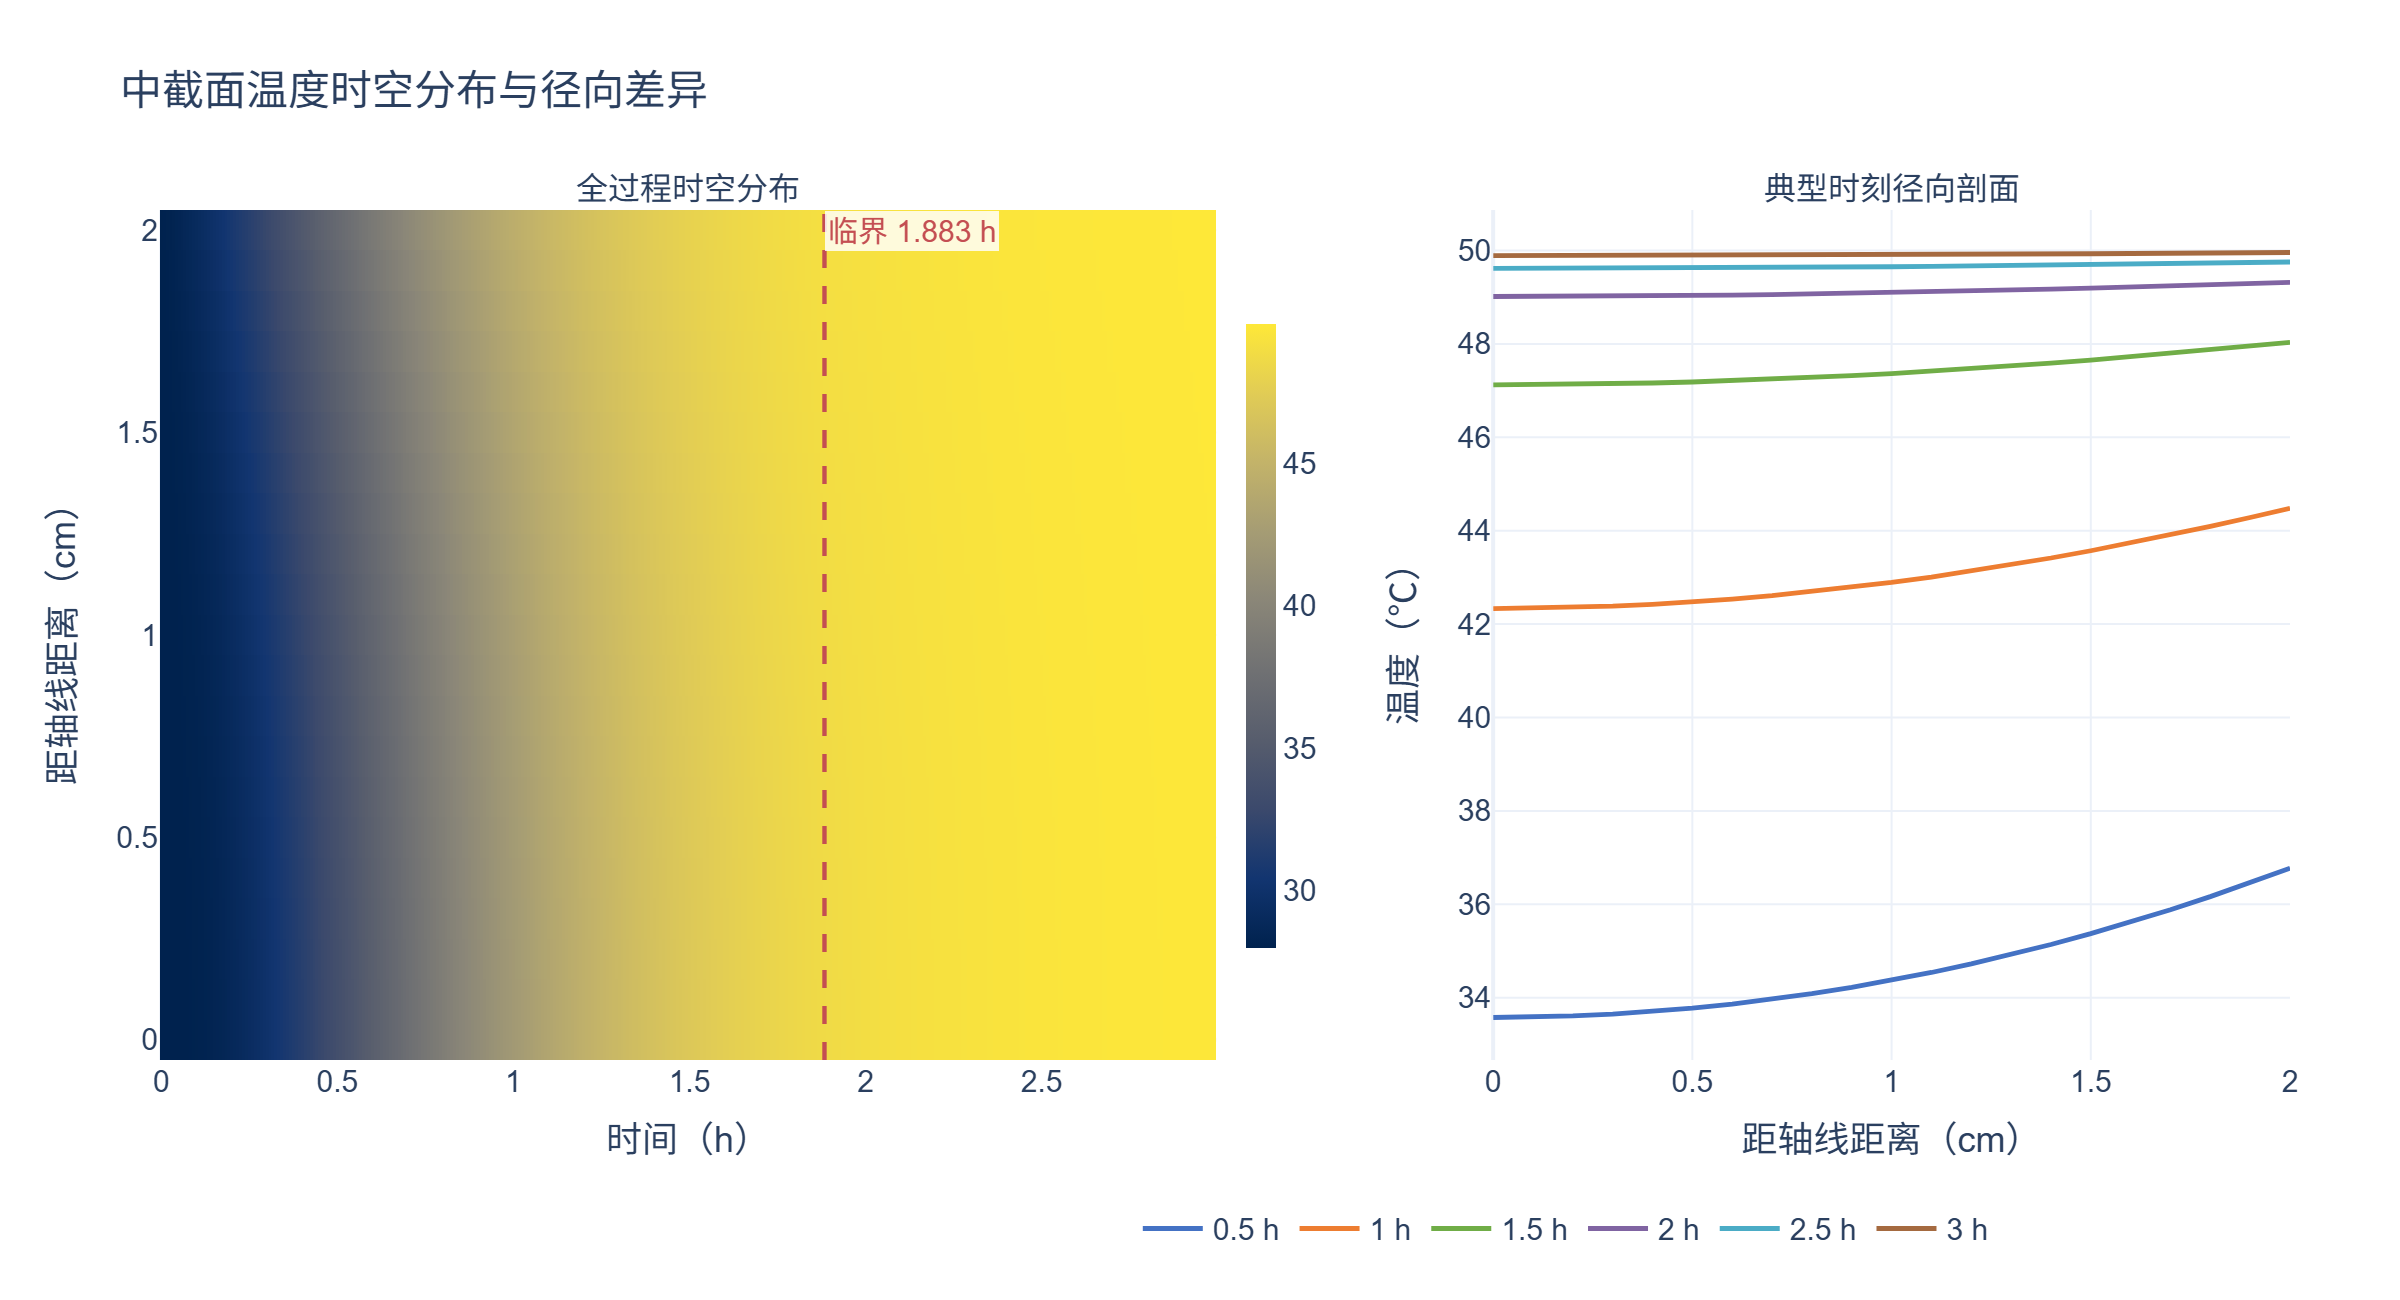
\includegraphics[width=0.98\textwidth]{graphics/fig_q2_temperature_field.png}
\caption{中截面温度时空分布与径向差异（左：全过程热力图，红色虚线为 $6780\ \mathrm{s}$ 的阶段分界；
右：六个典型时刻的径向剖面）}
\label{fig:p2temp}
\end{figure}

\begin{figure}[H]
\centering
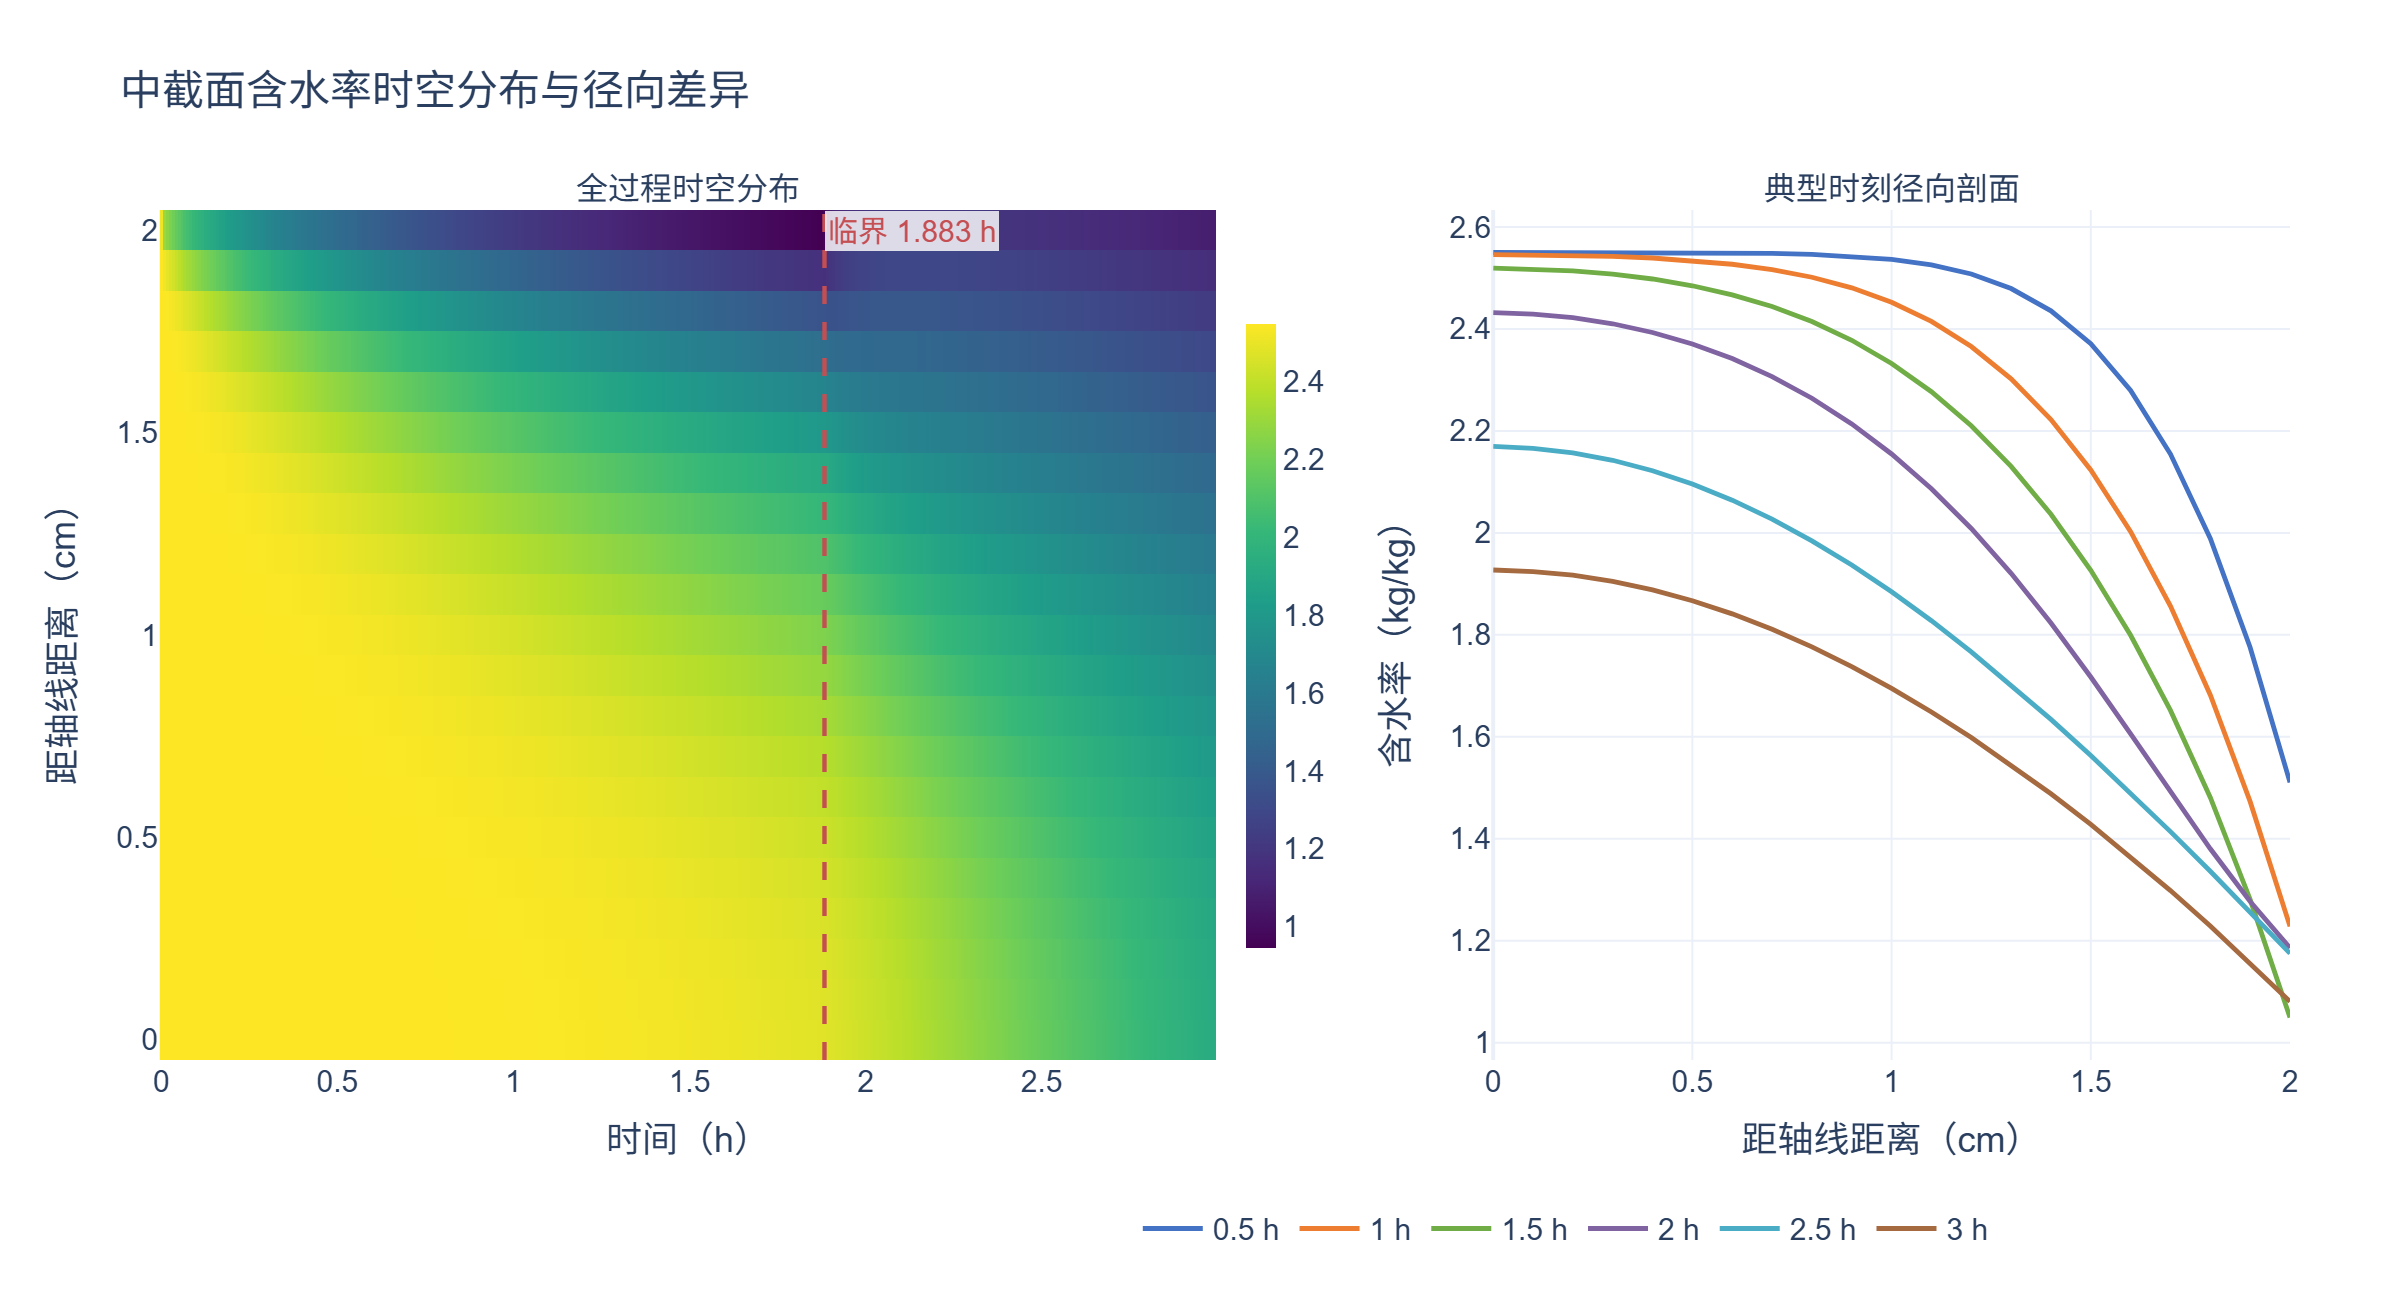
\includegraphics[width=0.98\textwidth]{graphics/fig_q2_moisture_field.png}
\caption{中截面含水率时空分布与径向差异（左：全过程热力图，红色虚线为 $6780\ \mathrm{s}$ 的阶段分界；
右：六个典型时刻的径向剖面）}
\label{fig:p2moist}
\end{figure}

\textbf{3. 结果分析}

\textbf{（1）阶段分界的影响。}临界点 $6780\ \mathrm{s}=1.8833\ \mathrm{h}$ 位于 $1.5\ \mathrm{h}$
与 $2.0\ \mathrm{h}$ 之间，因此前 $3\ \mathrm{h}$ 的结果中，前 $1.5\ \mathrm{h}$ 完全由预热
平衡参数主导，$2.0\ \mathrm{h}$ 之后开始包含恒温干燥参数的作用。由表~\ref{tab:T2} 可见，
$1.5\ \mathrm{h}$ 至 $2.0\ \mathrm{h}$ 之间中心温度由 $47.1226\ ^\circ\mathrm{C}$ 升至
$49.0152\ ^\circ\mathrm{C}$，升温速率已明显放缓，与烘房温度趋于恒定的过程一致。

\textbf{（2）温度场。}药材温度整体由侧面与端面向内部传递，早期径向温差显著、随后趋于均匀：
$0.5\ \mathrm{h}$ 时表面与中心的温差达 $36.7750-33.5769=3.20\ ^\circ\mathrm{C}$，
至 $3.0\ \mathrm{h}$ 已收缩至 $49.9594-49.8952=0.06\ ^\circ\mathrm{C}$。$3\ \mathrm{h}$ 时
中心温度 $49.8952\ ^\circ\mathrm{C}$、侧面温度 $49.9594\ ^\circ\mathrm{C}$，均与烘房平台温度
$50\ ^\circ\mathrm{C}$ 相差不足 $0.11\ ^\circ\mathrm{C}$，说明预热阶段结束时药材已基本热透，
温度场接近均匀，此后温度对水分迁移的影响主要通过 $D$ 的 Arrhenius 项体现。由图~\ref{fig:p2temp}
的热力图可见，色带以竖直方向（等温线沿轴向）为主，说明温度差异主要沿径向发展；临界时刻虚线
两侧颜色平滑过渡，表明临界点处只切换物性参数、温度场本身保持连续，不出现跳跃。右图的径向
剖面进一步给出直观的对比：$0.5\ \mathrm{h}$ 时曲线明显上翘（中心低、表面高），$1\ \mathrm{h}$、
$1.5\ \mathrm{h}$ 曲线依次抬升并趋于平缓，至 $2\ \mathrm{h}$ 以后各条曲线已彼此接近且几乎水平，
反映温度场由“外热内冷”逐步走向均匀。

\textbf{（3）水分浓度场。}水分浓度呈现明显的“内湿外干”径向梯度：$3\ \mathrm{h}$ 时中心
含水率为 $1.9237\ \mathrm{kg/kg}$，而侧面已降至 $1.0791\ \mathrm{kg/kg}$，径向差值达
$0.84\ \mathrm{kg/kg}$。这是因为表面失水由对流传质边界直接控制，而内部水分只能依靠扩散
缓慢外移，后者是控速环节。由图~\ref{fig:p2moist} 的热力图可见，色带以水平方向为主且左侧
（近轴线）始终偏黄、右侧（近表面）逐渐转深，说明含水率梯度主要沿径向分布；随时间的推进
整体颜色由黄转青、由青转紫，即含水率全断面整体下降。右图的径向剖面呈典型的“内高外低”
下凹形状，且随时间的推进整条曲线依次下移：$0.5\ \mathrm{h}$ 时曲线只在最外侧明显下落，
$2\ \mathrm{h}$、$3\ \mathrm{h}$ 时连中心区域也开始下降，说明干燥过程由表及里逐步推进。
临界时刻虚线两侧色带连续，与温度场一样未出现重置或跳变。

需要注意的是，表~\ref{tab:C2} 中$r=2\ \mathrm{cm}$（侧面）处的含水率并非单调下降，而是在
$1.05\sim1.51\ \mathrm{kg/kg}$ 之间波动。这是由侧面值需经对流边界条件~\eqref{eq:p2bc} 反解、
而其中的传质系数 $h_m$、扩散系数 $D$ 与烘房空气含湿量 $C_a(t)$ 均在时段内变化所致；同时
$t_c$ 前后的分段物性切换也会使表层薄层的平衡值发生小幅度调整。径向内侧（$r\le1.5\ \mathrm{cm}$）
的含水率则始终单调下降，不受该边界处理影响，符合物理预期。

\textbf{（4）判据的适用性。}本文将“是否进入恒温阶段”的判定建立在平台接近程度、升温斜率与
持续时间三项证据上，比单一进度阈值更能抵抗测温波动。但阈值 $2\sigma$、$3\sigma/\text{窗长}$
以及 $20/30$ 分钟的时间参数仍是建模选择，正式应用时应结合设备的控温精度与工艺容差做灵敏度
检验。

% =====================================================================
% 六、模型评价
% =====================================================================
\section{模型优缺点分析}
\subsection{优点}
\begin{itemize}
    \item 优点一……
    \item 优点二……
\end{itemize}
\subsection{缺点}
\begin{itemize}
    \item 缺点一……
    \item 改进方向……
\end{itemize}

% =====================================================================
% 参考文献
% =====================================================================

\begin{thebibliography}{99}

\raggedright

\bibitem{ref1}
SILVA W.P.da, SILVA C.M.D.P.S e, GAMA F.J.A. Estimation of thermo-
physical properties of products with cylindrical shape during drying: the coupling between mass and heat[J]. 
Journal of Food Engineering, 2014, 141: 65-73. DOI: 10.1016/j.jfoodeng.2014.05.010.

\bibitem{ref2}
COMSOL. Modeling with PDEs: Coordinate Transformations[EB/OL].
COMSOL Learning Center, 2026[2026-09-10].
\url{https://www.comsol.com/support/learning-center/article/modeling-with-pdes-coordinate-transformations-47951}

\bibitem{ref3}
CRANK J.
The Mathematics of Diffusion[M].
2nd ed. Oxford: Clarendon Press, 1975.

\bibitem{ref4}
CRANK J, NICOLSON P. A practical method for numerical evaluation of solutions of partial differential equations of the heat-conduction type[J]. Mathematical Proceedings of the Cambridge Philosophical Society, 1947, 43(1): 50-67. DOI:10.1017/S0305004100023197.

\end{thebibliography}

% =====================================================================
% 附录
% =====================================================================
\appendix
\renewcommand{\thesubsection}{\thesection.\arabic{subsection}}   % 附录子节编号为 A.1 而非 1.1
\section{附录}

% —— 支撑材料目录 ——
\subsection{支撑材料目录}
\begin{table}[H]
\centering
\begin{tabular}{ll}
\toprule
\textbf{文件名} & \textbf{功能说明} \\
\midrule
论文.pdf & 论文正文 \\
solve\_problem1.py & 问题一模型求解代码 \\
solve\_result2.py / plot\_results.py & 问题二模型求解与绘图代码 \\
result1.xlsx & 问题一结果表 \\
result2.xlsx & 问题二结果表 \\
\bottomrule
\end{tabular}
\caption{支撑材料目录}
\end{table}

% —— 核心代码（用 verbatim 或 lstlisting 展示，建议放关键的几段即可）——
\subsection{核心代码}
\begin{lstlisting}[language=Python, caption={代码说明（示例）}]
import numpy as np

def f(x):
    return np.sum(x ** 2)

print(f(np.array([1.0, 2.0, 3.0])))
\end{lstlisting}

\end{document}
